\documentclass{report}
\usepackage[utf8]{inputenc}
\usepackage[
backend=biber, 
style=ieee
]{biblatex}
\usepackage{listings}
\usepackage{hyperref}

\usepackage[utf8]{inputenc}
\usepackage{graphicx}
\usepackage[export]{adjustbox}

\usepackage{a4wide}

\title{Project Plan for CSE2000}
\author{K. Kanniainen, P. Ulev, Y. Wang, D. Coban, M. Cristea-Enache}
\date{1 May 2020}
      
\addbibresource{literature.bib} %Imports bibliography file

\begin{document}
\maketitle



\tableofcontents{}

\chapter{Introduction}
\section{Background}
Bacteria, microscopic, single-celled organisms, thrive and appear in many different environments such as in the soil, in the air, and in human bodies. In regard to their DNA, the concept of species is quite vague: some species are made up of nearly identical genomes, while in other cases the whole species shares about half of their total genome content. Keeping in mind that some of those strains could pose great danger to human health, the bioinformatics field is rapidly developing software to classify and identify each strain with high accuracy and recall \cite{mpgprimer}.


\section{Client goal}
With this background in mind, Delft Bioinformatics Lab wants us to develop a more streamlined and intuitive workflow that will enable more biologists to run their DNA analysis with little programming knowledge. The challenge lies in gathering the latest researched algorithms and combining them in an end-to-end, easy-to-use pipeline. More details about the goals and the list of features will be made clear in the requirements chapter.

\section {Approach}
To ensure a successful end product, our team has started the project with an orientation phase. More precisely, we have spent two weeks in which we have analysed the existing software solutions and interviewed key stakeholders. Furthermore, we have gathered and compared the benefits and drawbacks of the available tools, languages, and architecture choices. Last but not least, we have created a preliminary implementation timeline that will help us with assessing our progress during the development phase.


\section {Structure of this document}
As part of our two-week orientation phase, this project plan documents the research and design choices we have made. 

Chapter 2 contains a more detailed description of the problem put forward by the client and an analysis of the existing tools and algorithms that could help us build a good end product.

In Chapter 3 we describe the list of features we plan to implement. 

Chapter 4 is about the initial choices we have made, both in regard to technical tools and design principles, how we have made those decisions, and the risks we acknowledge.

Finally, Chapter 5 contains a preliminary implementation plan, including a week by week guideline schedule of the features.






































% Chapter 2
% Problem analysis (literature study)

\chapter{Problem analysis}
In this chapter we discuss the problem posed to us, considering some of the existing approaches and exploring why there is still work to be done.


\section{Background}
Often the significant genetic variation even within a single species can have a big impact over the properties of microbes. Different strains, when colonising a hospitalised patient for instance, should be treated in different ways and pose different levels of danger to begin with. This is why it is useful to be able to identify, as accurately and as quickly as possible, different strains of bacteria present in a sample \cite{mbs:/content/journal/mgen/10.1099/mgen.0.000075}. 

Modern technologies make it possible to easily extract DNA information from samples, but the limitation is that these methods cut the original DNA molecules into small fragments \cite{mpgprimer}.


\section{Problem statement and key goals}
Our challenge revolves around a computationally efficient tool to identify different strains of bacteria present in a sample of small DNA fragments. We have been asked to develop an end-to-end pipeline which can, given such a sample, estimate the relative abundances of bacterial strains present in the data. Our product should be easy to use for a scientist with limited computer science experience. Preferably, it should run on a cloud platform.

Input data may be given in the form of an identifier or a file path. Our product should download the data if it is not available in local storage already.

The pipeline should then proceed to estimate the strain abundances using initially an existing analysis tool and later on possibly our own implementation. The design should be modular so that the exact algorithms are interchangeable.

In the end, the results should be presented in a way that allows the users to easily draw conclusions from it.


\section{Existing end-to-end products} \label{end-to-end}

The following section will compare some existing tools for metagenomic analysis in terms of their output formats, speed and space efficiency, easiness of use and platforms they run on. We find Sigma \cite{ahn2015sigma}, Bib \cite{mbs:/content/journal/mgen/10.1099/mgen.0.000075}, StrainEst \cite{StrainEst}, and StrainSeeker \cite{roosaare2017strainseeker} most useful for our purpose. Note that the comparison significantly relies on the respective articles about these tools.

\textbf{Output}: it is the result of the calculations made by the algorithms in some kind of output files. StrainEst generates four text files and one pdf visualization file. They represent relative abundance and prediction information. Sigma generates one text and one html file. Both of them contain information about the estimation of the relative abundances. BIB generates only one file abundance.m\textunderscore alphas, which contains estimation of the strains and their abundances. StrainSeeker output will be shown in text including the identified strains marked as "KNOWN" or"RELATED" to the database genome, or a pie chart with the relative abundance of each strain.

\textbf{Speed and space efficiency}: BIB typically runs for around 10 minutes on 1M reads on a single-CPU PC. We tested StrainEst and it ran for around 30 minutes in a Docker container analysing a 28MB fastq file. Sigma is written in C++ and has a specific focus on speed, parallelisation and memory optimisation. It uses significantly less memory and has lower runtime than other tools (e.g. Pathoscope, MEGAN) \cite{ahn2015sigma}. It took Sigma 10 minutes and 10000 cores to complete the alignment step in their algorithm. However, Sigma took 1000 times computation time than StrainSeeker, when they are run on a single CPU core computer \cite{roosaare2017strainseeker}. StrainSeeker can have 1 Gb of data analysed in several minutes \cite{roosaare2017strainseeker}. But it needs at least 200 GB of HDD to build a customised database, where their default database takes up 4.5 GB or 18.5 GB of memory to download.

\textbf{Environments}:
on high-level, all four of these are just some folder with script files. They can be put in an isolated environment, such as a Docker container. StrainEst already has a dedicated Docker container for it \cite{strainest_docker}, with all the required tools installed in it. Similar Docker containers can be made for Sigma and BIB, and it is also possible to make one container containing all three of the tools and run them as needed. Terra supports Docker containers and automatically delegates all data and computation jobs to the integrated cloud service. 

\textbf{Usability}: some basic command-line competence is required to be able to work with the downloadable version of these programs. A programmer or a computational biologist should be able to make use of any of them, possibly requiring some time spent researching the APIs. As mentioned, StrainEst contains a set up environment with all the configuration done and additional tools downloaded. It is the most intuitive and easy to get started with, which in many cases is a vital step in choosing which tool to use for any kind of analysis. As far as we know, StrainSeeker is one of the few tools offering the online version of strain estimation. However, on StrainEst web version, the maximum size of metagenomic dataset the user can upload through their website is only 500MB and the web tool does not offer the option of customising the database. Therefore, the web version of their tool does not offer as much flexibility as their downloadable tool in terms of research purpose.


\section {Pipeline}
A pipeline in a Unix shell context consists of several commands linked to each other with a pipe ('$|$') character. This syntax connects the previous command or program's standard out to the next one's standard in to form a "pipe" of data flow. In a bioinformatics context, it means a similar system of analysis and data wrangling tools and commands, but is typically crafted with a dedicated description language that is more human-readable than simple bash and, aside the basic linear chaining, allows for various other "plumbing" settings, that is, data flow configurations such as branches and merges. These enable concurrent execution of suitable tools \cite{wdl}.

These core pipelines can be extended from both ends. In the front-end it is possible to abstract away code and ask the user for data sources and selected options with a graphical user interface. In the other end of the system, the results of the process can also be displayed visually without requiring any further interaction from the user.

A good pipeline should be modular. This means that each part in the pipeline should be replaceable with any piece of software that implements the same interface. In our project, the parts most likely to be replaced frequently are the exact analysis tools and the (cloud) platforms they should run on.


\subsection{Key features}
\begin{enumerate}
    \item User starts with a simple graphical user interface (GUI) to select a strain estimation tool and provide the sample data.
    \item A cloud platform will run the specified algorithm on the data. The data and algorithms used in the tasks can either be located on the same cloud platform or somewhere else.
    \item Once the computation is done, a report is displayed. It should provide a visually clear representation of the output data and options to download it.
\end{enumerate}


\subsection{Related tools}
This section presents some useful software tools that could be of use for our project. 

\textbf{WDL} (Workflow Description Language) is a language made to describe data processing workflows in a human-readable way. The syntax is user-friendly and structured and is appropriate for non-programmers as well. It can chain numerous tasks together and parallelise their execution. It is appropriate for genome analysis pipelines and developed by Broad Institute and has various tutorials online which further incited us to use it as our workflow language. WDL is not executable by itself, instead it needs to be run on an execution engine such as Cromwell \cite{wdl}.

\textbf{Snakemake} is one of the most famous workflow management system tools out there. Workflows are described with a human readable language based on Python and can be run on clouds, servers, and other environments. Its documentation is more extensive than WDL's and it is highly popular with its 591 citations, as of April 2020 \cite{dimensions}. Snakemake is widely used in bioinformatics and "interoperates ...  with any web service with well-defined input and output  (file) formats \cite{snakemake}."


\section {Algorithm}
The computational problem regarding strain identification is as follows: the input data consists of short DNA fragments extracted from the sample, while we also have a reference database containing information about known strains and their DNA profiles. 

A statistical model estimating the "mix" of different strains in a sample can be formulated as a multivariate linear regression problem. To formulate this, we first need a measure of similarity. One technique to estimate this revolves around k-mers, which are sequences of length k that are captured from the DNA fragments with a sliding window. The counts of different k-mers can be used as a measure of similarity between genomes and this will serve as the basis for our computation model. Further data analysis techniques may be used to improve accuracy.

The question of computational efficiency comes into play when the size of the sample data and the value of k are considered. The input datasets are typically big, even hundreds of gigabytes, so we cannot rely on fitting everything in the main memory at once; instead, we will want to design an algorithm that processes the data one row at a time. Furthermore, there are $4^k$ possible k-mers in a DNA sequence, as every character in the k-mer can be any of the four bases A, C, T, and G. As we have to track a count for each of these, we need to pick sufficiently small values for k.


\subsection{Existing algorithms}
This section explains the key steps used in the 3 existing algorithms mentioned in section \ref{end-to-end}. Their way of how to approach and how to solve the problem as well as which tools to use may serve a good reference when we create our own algorithm.

\textbf{Sigma} algorithm \cite{ahn2015sigma} for metagenomic biosurveillance uses a stochastic probabilistic model to resemble metagenomic reads sampling from genomes. In order to align metagenomic reads against reference genomes, Sigma adopted a short-read alignment algorithm, Bowtie2 \cite{Bowtie}, by default. To estimate the probability of sampling a random read from the reference genome $g_j$, Sigma uses the non-linear programming method implemented in the Ipopt library \cite{Ipopt}. 

\textbf{StrainEst} \cite{StrainEst} is a program that uses single-nucleotide variants (SNV) profiles to count and identify coexisting strains and their relative abundances. The pairwise Mash distances \cite{Mash} are computed between the genomes of the species of user interest and the species representative (SR), in order to filter out unrelated genomes. They use complete linkage hierarchical clustering to select the representative set of genomes, which are aligned onto SR using MUMmer\cite{MUMmer} and the SNV profiles are calculated. 10 representative genomes of the species are selected and aligned with reads using Bowtie2 \cite{Bowtie}. Given the SNV profiles, Lasso regression is used to identify the reference strains as well as their relative frequencies which fit best into the observed allelic frequencies. 

\textbf{BIB}, Bayesian identification of bacterial strains from sequencing data \cite{mbs:/content/journal/mgen/10.1099/mgen.0.000075}, uses UPGMA method in the MEGA6 \cite{MEGA6} to cluster the strains and uses progressiveMauve \cite{progressive} for multiple sequence alignment, in order to selects reference genomes. Then, BIB uses Bowtie2 \cite{Bowtie} to let the reads align against the reference sequences. BitSeq \cite{bitSeq} is used to estimate the relative frequency of each strain in the sequenced dataset.


\subsection{Related tools} 
This section features some genomic analysis tools that could be used in our algorithm.

\textbf{Mash} is an alignment-free toolkit to compute the distance between two genome sequences. It extends the MinHash algorithm, which compresses large sequences to sketch representations. Mash then compares the sketches and computes the Jaccard index, the proportion of shared k-mers, acting as a significance value for the match, and the Mash distance, which assesses proportion of the mutation between two sequences \cite{Mash}.

\textbf{Tensorflow} is a machine learning library, mostly used for image processing, reinforcement learning and time-series analysis \cite{tensorflow_article}. It has a powerful and complex set of tools and features with a good API. Its main focus are different types of neural networks and many kinds of real-world problems can be solved with it. Google developers work on it and it currently has state-of-the art novel algorithms in machine learning. It is also well-known for the ability to operate on large scale environments. Tensorflow is available in multiple languages, including Python, Javascript, C++, and Java.


\section{Cloud platforms}
Cloud computing is a large area of research nowadays. It is helpful in numerous fields, including bioinformatics, as the file sizes can be quite big and the algorithms used often require a considerable amount of computational power; cloud environments are built to scale as needed.

The expected user group of our program is biologists. We expect them to have either none or a very basic understanding of programming, so a cloud-native solution with an intuitive workflow that does not require the end user to install software themselves could be really useful and we have not encountered such a tool in our research this far. Another upside is that cloud-native workflows are very easy to share to the larger scientific community. This significantly improves the impact potential of our work.

For these reasons as well as being one of the goals put forward by our client, we have researched one of the cloud platforms used by the bioinformatics community.


\subsection{Terra}
The cloud platform Terra allows users to upload their data to the cloud and lets them use each other's published workflows combined with applications like Jupyter Notebook within a simple interface. It has built-in support for various genomic analysis tools. Cloud computing is also supported in the form of Google Cloud integration and the use of containers \cite{terra.bio, broad-institute}.

Terra offers native support for running scripts written in WDL \cite{terra.bio}. WDL in turn "... makes it straightforward to define complex analysis tasks, chain them together in workflows, and parallelize their execution" \cite{wdl}.





























% Chapter 3
% Requirements

\chapter{Requirements}
This chapter is dedicated to the features our team, in close collaboration with the client, has decided to implement. We briefly discuss the process of feature negotiation, followed by a list of functional and non-functional requirements. In the feasibility study section we motivate some prioritisations we have made.


\section{Methodology}
Using the MoSCoW prioritisation method \cite{clegg1994moscow}, we were able to reach an agreement with key stakeholders on the importance of each feature we might implement. The most important features are labelled into the \textbf{Must Have} category; the ones that are important but not as critical are grouped into the \textbf{Should Have} category. The requirements that are desirable but are not necessary for the program are grouped into the \textbf{Could Have} category, while the features in the \textbf{Won't Have} category will not be planned for during this timeframe.

We have also distinctly marked (with asterisks) some of the requirements in the following section: those requirements have an adjusted priority, which is a result of our feasibility study. We will go in more depth about how we made these choices, in agreement with our client, in section 3.4.


\section{Functional requirements}
These are requirements that concern the features of the software and can be represented as use cases.
\begin{enumerate}
    \item The program \textbf{must} be able to use sample and reference data residing on the same platform as the program.
    \item The program \textbf{must} be able to use at least one existing strain estimation tool to compute a prediction of the relative abundances of the strains present in the sample. \textbf{*}
    \item After the strains have been estimated the program \textbf{must} offer a report with the results in a standardised machine- and human-readable format.
    \item The program \textbf{must} offer a graphical user interface for uploading the required data, triggering the computations, and viewing the results. \textbf{**}
    
    \item The program \textbf{should} be able to use sample data from a public database, given an identifier.
    \item The program \textbf{should} offer the user a choice of multiple existing strain estimation tools. \textbf{*}
    \item The program \textbf{should} be able to use a reference genome database from a public database, given an identifier. \textbf{*}
    \item The program \textbf{should} offer a visualisation of the results.
    
    \item The program \textbf{could} offer the user the possibility of running multiple available strain estimation tools in parallel and displaying the results in a combined view. \textbf{*}
    \item The program \textbf{could} perform preprocessing on the input data, such as trimming the fragments, in order to increase accuracy. \textbf{*}
    \item The program \textbf{could} feature our own estimation process   alongside the existing ones. \textbf{*}
    
    \item The program \textbf{won't} offer the user the possibility of starting the workflow with downloading and building a relevant reference genome database by picking from a list of available species.
\end{enumerate}


\section{Non-functional requirements}
These requirements concern the properties and performance of the software that are not specific to any single use case.
\begin{enumerate}
    \item The software \textbf{must} include separate files for server-side and client-side code. \textbf{**}
    \item The written code \textbf{must} be readable and commented according to industry standard code formatting guidelines.
    \item The code \textbf{must} be tested where applicable, with branch coverage of at least 45 \%.
    
    \item The program \textbf{should} make use of a cloud platform to perform computations.
    \item The files \textbf{should} include documentation sufficient for a biologist to run the program.
    \item The code \textbf{should} have branch coverage of at least 75 \%.
    \item The code \textbf{should} have meaningful documentation for each class and method.
    \item The code \textbf{should} make use of modular design so that it is possible to add new algorithms later on.
    
    \item The program \textbf{could} make use of available genome analysis tools and other libraries such as GATK, Jellyfish, Mash, SciKit, and Pandas, in order to craft our own implementation of the strain identification process.
    \item The model fitting process \textbf{could} include cross-validation and other machine learning tools in order to avoid overfitting.
    \item The program \textbf{could} be available on a widely-used cloud platform, accessible to researchers in the field. \textbf{**}
    \item The software \textbf{could} include a workflow description written in a language that is commonly used in the field of bioinformatics. \textbf{**}
    
    \item The program \textbf{won't} offer significantly better accuracy than the existing state-of-the-art tools. \textbf{*}
    \item The program \textbf{won't} offer the user an option of using a cloud platform of their choice.
\end{enumerate}


\section{Feasibility study}
In this section we briefly discuss the process of requirement negotiation. Based on the key goals put forward by the client, we came up with an initial list of requirements, most of which can still be found in the previous section. However, after multiple interviews with key stakeholders, two rounds of changes had been made. Firstly, client desired a bigger priority on the pipeline than the algorithm. Second, after discussion with our teaching assistant and coach, we realised we should target a broader end user base. For this reason, we dropped developing a workflow for an existing bioinformatics platform in favour of developing a more intuitive and easy to use GUI.

As previously stated, the first adjustment our team had to make after reviewing and negotiating the requirements has been a shift of priority between the pipeline and the algorithm (the respective concepts of which we have analysed in depth in Chapter 2). The opinion of our client is that developing a better pipeline would be more preferable than a new fast and memory efficient algorithm. For this reason, we had shifted priorities: more pipeline features had gained a bigger priority while the algorithm features had lost priority. More so, we had been adding some of the client's suggestions as features our end product could contain. All of these changes can be seen in the list of requirements in the form of a single asterisk.

The second adjustment our team had to make was broadening the profile of the end user as per request of our coach. We have decided that the user should not need to leave the GUI but our program should automatically handle all interaction with external services instead. For this reason we dropped the requirement for creating a program in a workflow description language in favour of creating our own program, interacting independently of any specific cloud infrastructure. These changes are visible in the list of requirements, marked with 2 asterisks.

The changes we have made in our requirements have been on the cautious side. We consider it a better idea to mark more requirements as important but non-essential in order to not run out of time and resources for this project. With these requirements we are comfortable of finishing all \textbf{Must Haves}, most \textbf{Should Haves} and some \textbf{Could Haves} as the MoSCoW method imposes. 

%* -> shifted priority between pipeline and algorithm
%**-> gui focus changes


































% Chapter 4
% Project approach

\chapter{Project approach}
This chapter is dedicated to exploring several possible tools that we will use during our development phase. After finishing the list of requirements, our team has considered multiple choices in order to get the desired end product. Thus, each subsection contains a brief discussion about the tool we have chosen and the advantages over other possibilities.


\section{Development process framework}
One of the first choices we had to make was which development process framework to use. In broad terms, there are 2 main ways in which we can guide the process: a waterfall approach or an agile one.

The waterfall model \cite{royce1987managing} is based on minimizing risks through a systematic and thorough linear approach. More specifically, the waterfall model offers a structured approach, with clearly defined phases (requirements, design, implementation) while also emphasizing the importance of documentation. Its main drawbacks are the lack of working prototypes until late in the process as well as being unable to change the requirements during the implementation phase.

An agile approach \cite{fowler2001agile} supports an incremental, iterative process. It offers a working product throughout the whole project, slowly adding more features upon it. It promotes early and often collaboration between the client and the developers in order to build the best possible product. 

For these reasons, our team chose an agile approach, more specifically the Scrum process \cite{schwaber2004agile}. In order to adapt the scrum approach to our needs as best as possible we will work with one week long sprints; the planning for each sprint will happen on Monday morning and the retrospective on Friday afternoon. 


\section{Technological approach}
The existing tools to analyse metagenomic data-sets are quite hard to use and there is a need for a unified solution. For our program we decided to create an end-to-end solution to improve the user experience, so our solution will consist of a web application, a Docker container, and a cloud service to perform computations in a scalable way.

The web application will run on Node.js, which is a widely used JavaScript framework. It will offer both a simplified user interface and API endpoints for triggering the computations. We prefer Node over Spring, for instance, because of the good package manager `npm` for installing any dependencies and the added convenience of writing both the front-end and the back-end in the same language.

We will specify a standard for the output of the tool in close communication with the client to display relevant information about the results. This specification will help installing future algorithms to our tool.


\subsection{GUI frameworks}
We are going to use Vue.js as our front-end framework as we consider it to be the easiest to learn out of the well-documented front-end libraries available. Part of our team has previous experience with front-end JavaScript libraries, but we want our code base to be reasonably understandable for all of us.
 
The data visualisation view that shows the results of the process will make use of the Chart.js framework, which makes it easy to display all kinds of graphs from a dataset.


\subsection{Pipeline phases}
The steps to execute in the back-end are outlined as follows:
\begin{enumerate}
    \item get authorisation to use the user's cloud account,
    \item transfer the sample data to the cloud platform from the location specified by the user,
    \item send a command to the cloud platform to start computing,
    \item receive a "done" notification from the cloud platform and fetch the results,
    \item offer a report and visualisation on the results from the strain estimation tool.
\end{enumerate}


\subsection {Cloud platform}
There are three well-known cloud platforms that could be suitable for the task - Microsoft Azure, Google Cloud, and Amazon Web Services. Since there are no obvious differences in terms of features, we will make our decision based on available integration support. We will initially use AWS because there is a widely-used package for it on \texttt{npm}, \texttt{aws-sdk}, with over four and half million weekly downloads at the time of writing.

As a back-up plan, if it proves not feasible to use cloud services directly in the way we have planned, we will wrap the container in a WDL script and use Terra as an intermediary since it has Google Cloud integration pre-configured. Terra provides an API alongside the normal web interface.


\subsection{Docker container}
The computation will run on a customised Docker container that we will build as part of the project and publish on Docker Hub for easy access. The container will initially include one pre-installed strain estimation pipeline. We will keep the design modular so that adding another algorithm later on will be possible by installing it on the container, adapting the tool output to our specification, and adding the new algorithm to the GUI with any additional parameters needed to run this specific algorithm.

The container needs to run a widely-used operating system for the best compatibility. We chose the latest long term supported Ubuntu 18.04 LTS "Bionic Beaver" for this, as having a natively supported bash shell is highly useful and the native package manager `apt` makes installing dependencies quite easy.

The first strain estimation tool we will install on the container will be BIB \cite{mbs:/content/journal/mgen/10.1099/mgen.0.000075}. The steps needed to execute the pipeline are outlined as follows:
\begin{enumerate}
    \item build the reference genome database as specified, downloading the genomes as needed,
    \item execute the estimation process on the provided sample,
    \item convert the output file to our standard specification,
    \item trigger a webhook to indicate that the computation is finished.
\end{enumerate}


\subsection{Algorithm frameworks}
In the requirements, our own strain estimation algorithm is a "could have" feature, and we chose Python for this as the main programming language. Python is widely used for data analysis \cite{python_data_analysis} and machine learning problems. Its readable syntax and low complexity allow programmers to focus more on logic and less on implementation details. We consider this as a key factor. In addition, it has numerous libraries for really efficient mathematical operations, such as NumPy, which is particularly good at matrix manipulations, Pandas for dataframes, and matplotlib for visualisations. It also has good package manager (pip), which we can use to deal with external libraries. Python is therefore an appropriate choice for metagenomic analysis tasks.


\section{Quality assurance}
In our GitLab instance, the master branch is protected so that team members cannot push to it directly. Rather, we will update the code in our master branch with the Merge Request functionality by cross-reviewing each other's code. This will result in better code quality in our master branch. Pushes to all branches will trigger a continuous integration pipeline which executes tests and static analysis tools and notifies users on failure. A branch failing the pipeline cannot be merged.


\subsection{Software testing}
We do not plan on automating tests for the front-end, but the back-end Node.js server will be tested with the testing framework Mocha, where applicable. We will test any Python scripts we create for the project with the \texttt{py.test} module, which features a nice and simplistic syntax. Test coverage will be measured by the \texttt{Istanbul} and \texttt{pytest-cov} tools, respectively.


\subsection{Static analysis tools}
The code readability and quality in each file will be moderated by the appropriate tools for each file type; \texttt{eslint} for the JavaScript application and \texttt{pylint} for any Python files.


\subsection{Version control}
We are required to use the TU Delft's GitLab server for version control. It offers us an issue board, which we will use as a virtual Scrum board, while also supporting the basic git features. For writing the associated documentation, we use \LaTeX{} on the collaborating platform Overleaf.


\subsection{License}
The client required us to use Apache v2 as a license for this project \cite{apachev2}. Users of our software are able to use, modify or distribute source code on the condition that all original files carry a note stating the authorship as well as all changes made by the user in that particular file. However, the future users are able to select a different license for their changes and overall project.


\section {Risk analysis}
Two of the main risk factors during the process of implementing the software is communication within the group and communication with the client. To ensure we do not have problems with group level communication we have daily scrum meetings as well as a retrospective meetings at the end of each week. Additionally, we have weekly meetings with the teaching assistant to help us with any problems we might encounter. We also have weekly meetings with the client to ensure we are on track with what the client wants.

One risk factor in the planning stage of the project is the appropriateness of the requirements. Each group member conducted research after the client stated their goals for the end result of this project. Since none of the members of the group are bioinformatics experts, the end goal and how to achieve it were unclear and ambiguous at the start. Due to our limited understanding of bioinformatics and genomics, our requirements could prove to be unsatisfactory. This would result in the client not getting the program they asked for. On the opposite end of the spectrum, again due to our limited knowledge on the biology side of the project, if the requirements are too ambitious and not feasible the end product will be absent of the features the client wanted. 

One such feature is the algorithm. The algorithm could prove to be too difficult and time consuming to implement. Therefore, after consulting the client, we decided to first implement the core pipeline software and make it usable with existing algorithms. This way we limit the risk factor such that the client will get the pipeline they want immediately, and afterwards we might be developing the algorithm for the remainder of the project.


































\chapter{General planning for the remainder of the project}

After analysing the task that was given to us in Chapter 2, by clearly specifying the features we are going to implement and the tools we are going to use in Chapters 3 and 4, we are ready to start the development phase. 
 
By using the insight we have gathered and shared in this project plan, we feel ready to create the schedule we are going to follow for the remaining weeks. We are going to work in weekly sprints, having regular meetings to track our progress; not only within the team through the weekly retrospective but also with the client and our software project coach.
 
Taking inspiration from a project plan example the course coordinators have provided us \cite{examplereport}, we have created a week by week plan, attached below, highlighting when we will work on different parts of the product as well as various deadlines and course-related assignments. Green blocks represent the time our team will use to work on the product, red blocks represent deadlines our project has to follow and the blue blocks serve as reminders to start working on certain course assignments.

\begin{figure}
    \centering
    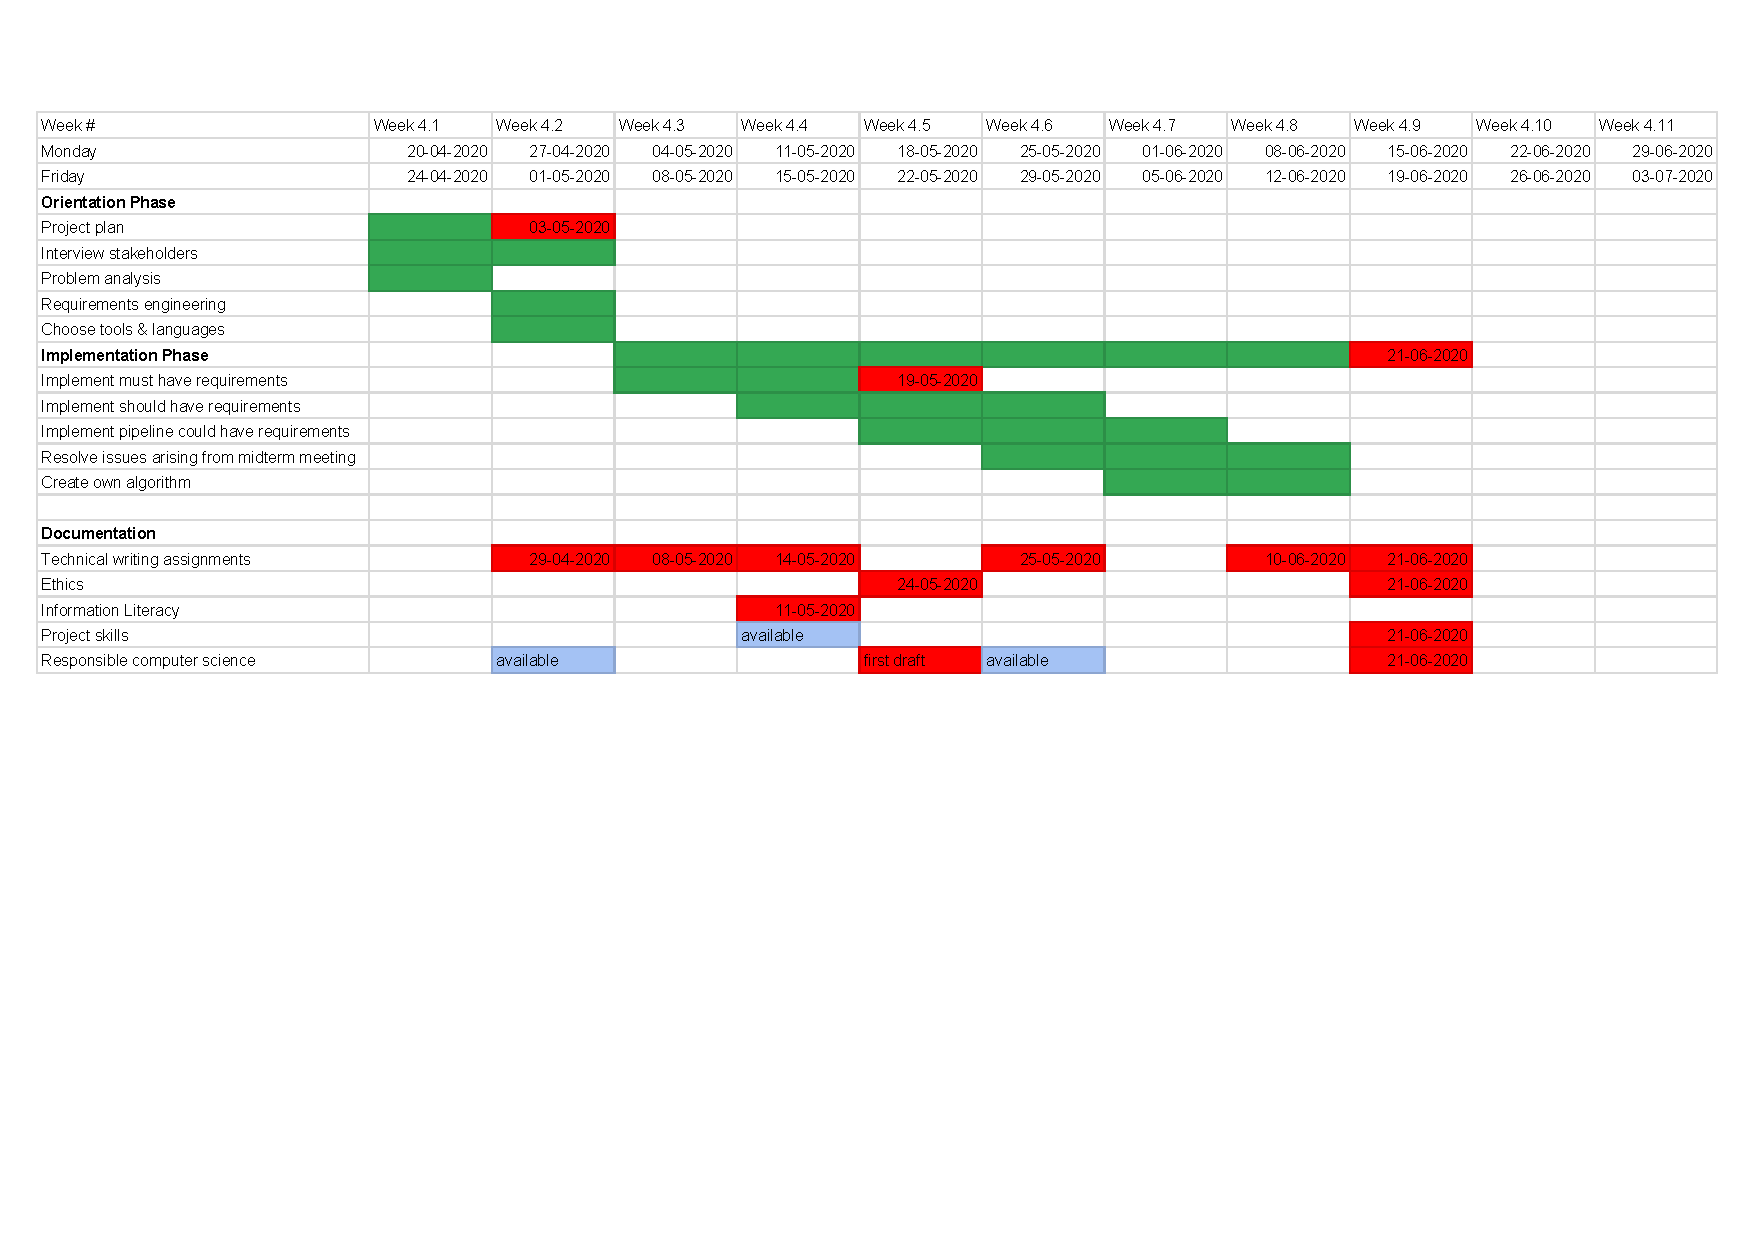
\includegraphics[width=17cm, left]{scheduling - Sheet1.pdf}
    \caption{General Planning}
    \label{planning}
\end{figure}


\medskip
\printbibliography
\end{document}
